% \documentclass[aspectratio=169,notes]{beamer}
\documentclass[aspectratio=169]{beamer}
\usetheme[faculty=phil]{fibeamer}
\usepackage{polyglossia}
\setmainlanguage{english} %% main locale instead of `english`, you
%% can typeset the presentation in either Czech or Slovak,
%% respectively.
\setotherlanguages{russian} %% The additional keys allow
%%
%%   \begin{otherlanguage}{czech}   ... \end{otherlanguage}
%%   \begin{otherlanguage}{slovak}  ... \end{otherlanguage}
%%
%% These macros specify information about the presentation
\title[AGLA1]{Analytical Geometry and Linear Algebra I, Lab 10} %% that will be typeset on the
\subtitle{Conic sections (2nd order curve equation): Hyperbola
\\ From general to canonical form  \\ Tangent line to a curve
         } %% title page.
\author{Oleg Bulichev}
%% These additional packages are used within the document:
\usepackage{ragged2e}  % `\justifying` text
\usepackage{booktabs}  % Tables
\usepackage{tabularx}
\usepackage{tikz}      % Diagrams
\usetikzlibrary{calc, shapes, backgrounds}
\usepackage{amsmath, amssymb}
\usepackage{url}       % `\url`s
\usepackage{listings}  % Code listings
% \usepackage{subfigure}
\usepackage{floatrow}
\usepackage{subcaption}
\usepackage{mathtools}
\usepackage{todonotes}
\usepackage{fontspec}
\usepackage{multicol}
\usepackage{pdfpages}
\usepackage{wrapfig}
\usepackage{animate}
\usepackage{booktabs}
\usepackage{multirow}

\newcommand{\shf}{\text{shift}}

\graphicspath{{resources/}}
\frenchspacing

\setbeamertemplate{caption}[numbered]
\usetikzlibrary{graphs}

% \usepackage[backend=biber,style=ieee,autocite=footnote]{biblatex}
% \addbibresource{biblio.bib}
% \DefineBibliographyStrings{english}{%
%   bibliography = {References},}

\newcommand{\oleg}[2][] {\todo[color=red, #1] {OLEG:\\ #2}}
\newcommand{\fbckg}[1]{\usebackgroundtemplate{\includegraphics[width=\paperwidth]{#1}}}%frame background

\usepackage[framemethod=TikZ]{mdframed}
\newcommand{\dbox}[1]{
\begin{mdframed}[roundcorner=3pt, backgroundcolor=yellow, linewidth=0]
\vspace{1mm}
{#1}
\vspace{1mm}
\end{mdframed}
}

\begin{document}
\setlength{\abovedisplayskip}{0pt}
\setlength{\belowdisplayskip}{0pt}
\setlength{\abovedisplayshortskip}{0pt}
\setlength{\belowdisplayshortskip}{0pt}

\fbckg{fibeamer/figs/title_page.png}
\frame[c]{\setcounter{framenumber}{0}
    \usebeamerfont{title}%
    \usebeamercolor[fg]{title}%
    \begin{minipage}[b][6.5\baselineskip][b]{\textwidth}%
        \textcolor{black}{\raggedright\inserttitle}
    \end{minipage}
    % \vskip-1.5\baselineskip

    \usebeamerfont{subtitle}%
    \usebeamercolor[fg]{framesubtitle}%
    \begin{minipage}[b][3\baselineskip][b]{\textwidth}
        \raggedright%
        \insertsubtitle%
    \end{minipage}
    \vskip.25\baselineskip
}
%   \frame[c]{\maketitle}
\note{
    \begin{enumerate}
        \item Теперь потренируем в каноникал, когда есть поворот.
        \item С тангент, берем сложную производную и все чики пуки

    \end{enumerate}
}

\fbckg{fibeamer/figs/common.png}


% \begin{frame}[c]{Questions from the class}
%     \framesubtitle{}
%     \centering
%     \textit{ \Large No questions for today}
% \end{frame}

\begin{frame}[t]{Questions for today}
    \framesubtitle{}
    \begin{itemize}
        \item How can I work with general form of 2nd order curve equation?
        \item How it relates with cone?
        \item What forms of equation do we have?
    \end{itemize}
\end{frame}


\begin{frame}[t]{Some definitions, which can be helpful}
\framesubtitle{Eccentricity, Directrix}
    \begin{columns}[T,onlytextwidth]
        \begin{column}{0.59\textwidth}
            \textbf{Eccentricity} is a measure of how much a conic section deviates from being circular. \medskip
        
            It is a constant ration between distance from focal to point on the curve and from the point on the curve to \textbf{directrix}.
        \end{column}
        \begin{column}{0.39\textwidth}
            \vspace{-1cm}
            \begin{figure}[H]
                    \centering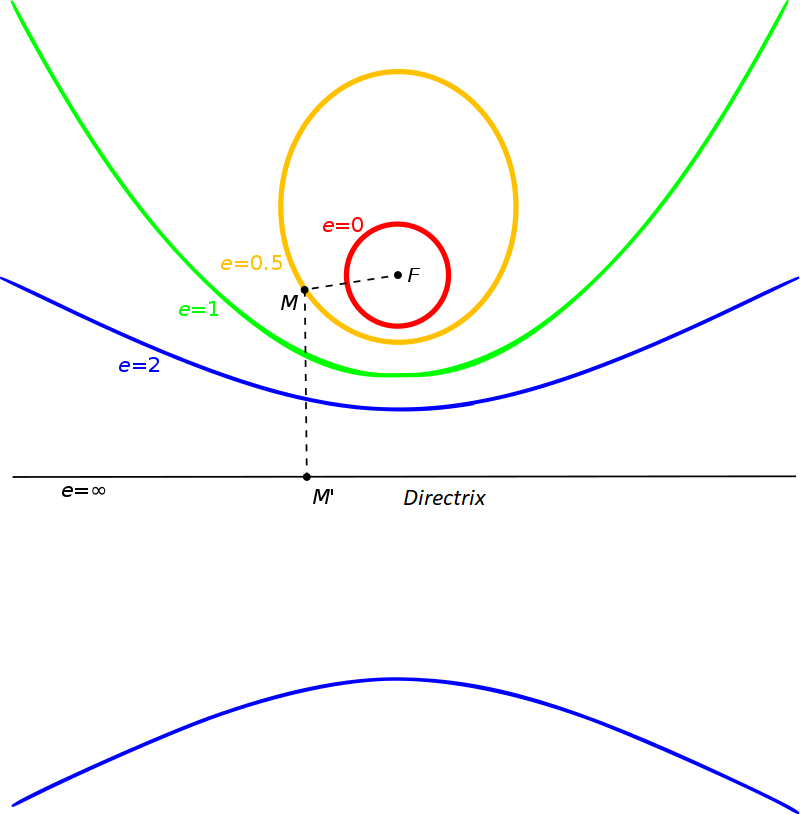
\includegraphics[height=7cm,width=1\textwidth,keepaspectratio]{eccentricity.png}
                    % \caption{capture1}
                    \label{fig:eccentricity.png}
            \end{figure}
        \end{column}
    \end{columns}
\end{frame}

\begin{frame}[t]{Some definitions, which can be helpful}
\framesubtitle{Linear eccentricity, Latus Rectrum, Focal parameter}
    \begin{columns}[T,onlytextwidth]
        \begin{column}{0.59\textwidth}
            The \textbf{linear eccentricity} is the distance between the center and the focus (or one of the two foci). \medskip 
            
            The \textbf{latus rectum} is the chord parallel to the directrix and passing through the focus (or one of the two foci). \medskip 
            
            The \textbf{focal parameter} is the distance from the focus (or one of the two foci) to the directrix.

        \end{column}
        \begin{column}{0.39\textwidth}
            \vspace{-1cm}
            \begin{figure}[H]
                \begin{subfigure}{0.99\textwidth}
                    \centering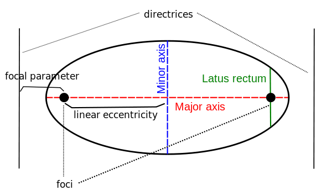
\includegraphics[height=4cm,width=1\textwidth,keepaspectratio]{ellipse_focal.png}
                    % \caption{capture1}
                    \label{fig:ellipse_focal.png}
                \end{subfigure}

                \begin{subfigure}{0.99\textwidth}
                    \vspace{-0.6cm}
                    \centering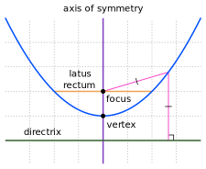
\includegraphics[height=3cm,width=1\textwidth,keepaspectratio]{parabola_focus.png}
                    % \caption{capture2}
                    \label{fig:parabola_focus.png}
                \end{subfigure}
            % \caption{capture_main}
            % \label{fig:}
            \end{figure}
        \end{column}
    \end{columns}
\end{frame}

\begin{frame}[t]{Parabola}
    \framesubtitle{}
        \scriptsize
        \vspace{-0.4cm}
    \begin{columns}[T,onlytextwidth]
        \begin{column}{0.59\textwidth}
            \textit{Forms:} \\
    \begin{itemize}
        \item \textbf{Canonical (should be w/o shift)} $(x-x_{\shf})^2=2p(y-y_{\shf})$
        \item \textbf{General} $Ax^2+Bxy+Cy^2+Dx+Ey+F=0$, where either $A=0$ or $C=0$, not both, if $B=0$
        \item \textbf{Parametric} $\left\{\begin{matrix*}[l] x = \sqrt{2}pt\\ y = pt^2\end{matrix*}\right.$
    \end{itemize}
        \end{column}
        \begin{column}{0.39\textwidth}
            \begin{figure}[H]
                \centering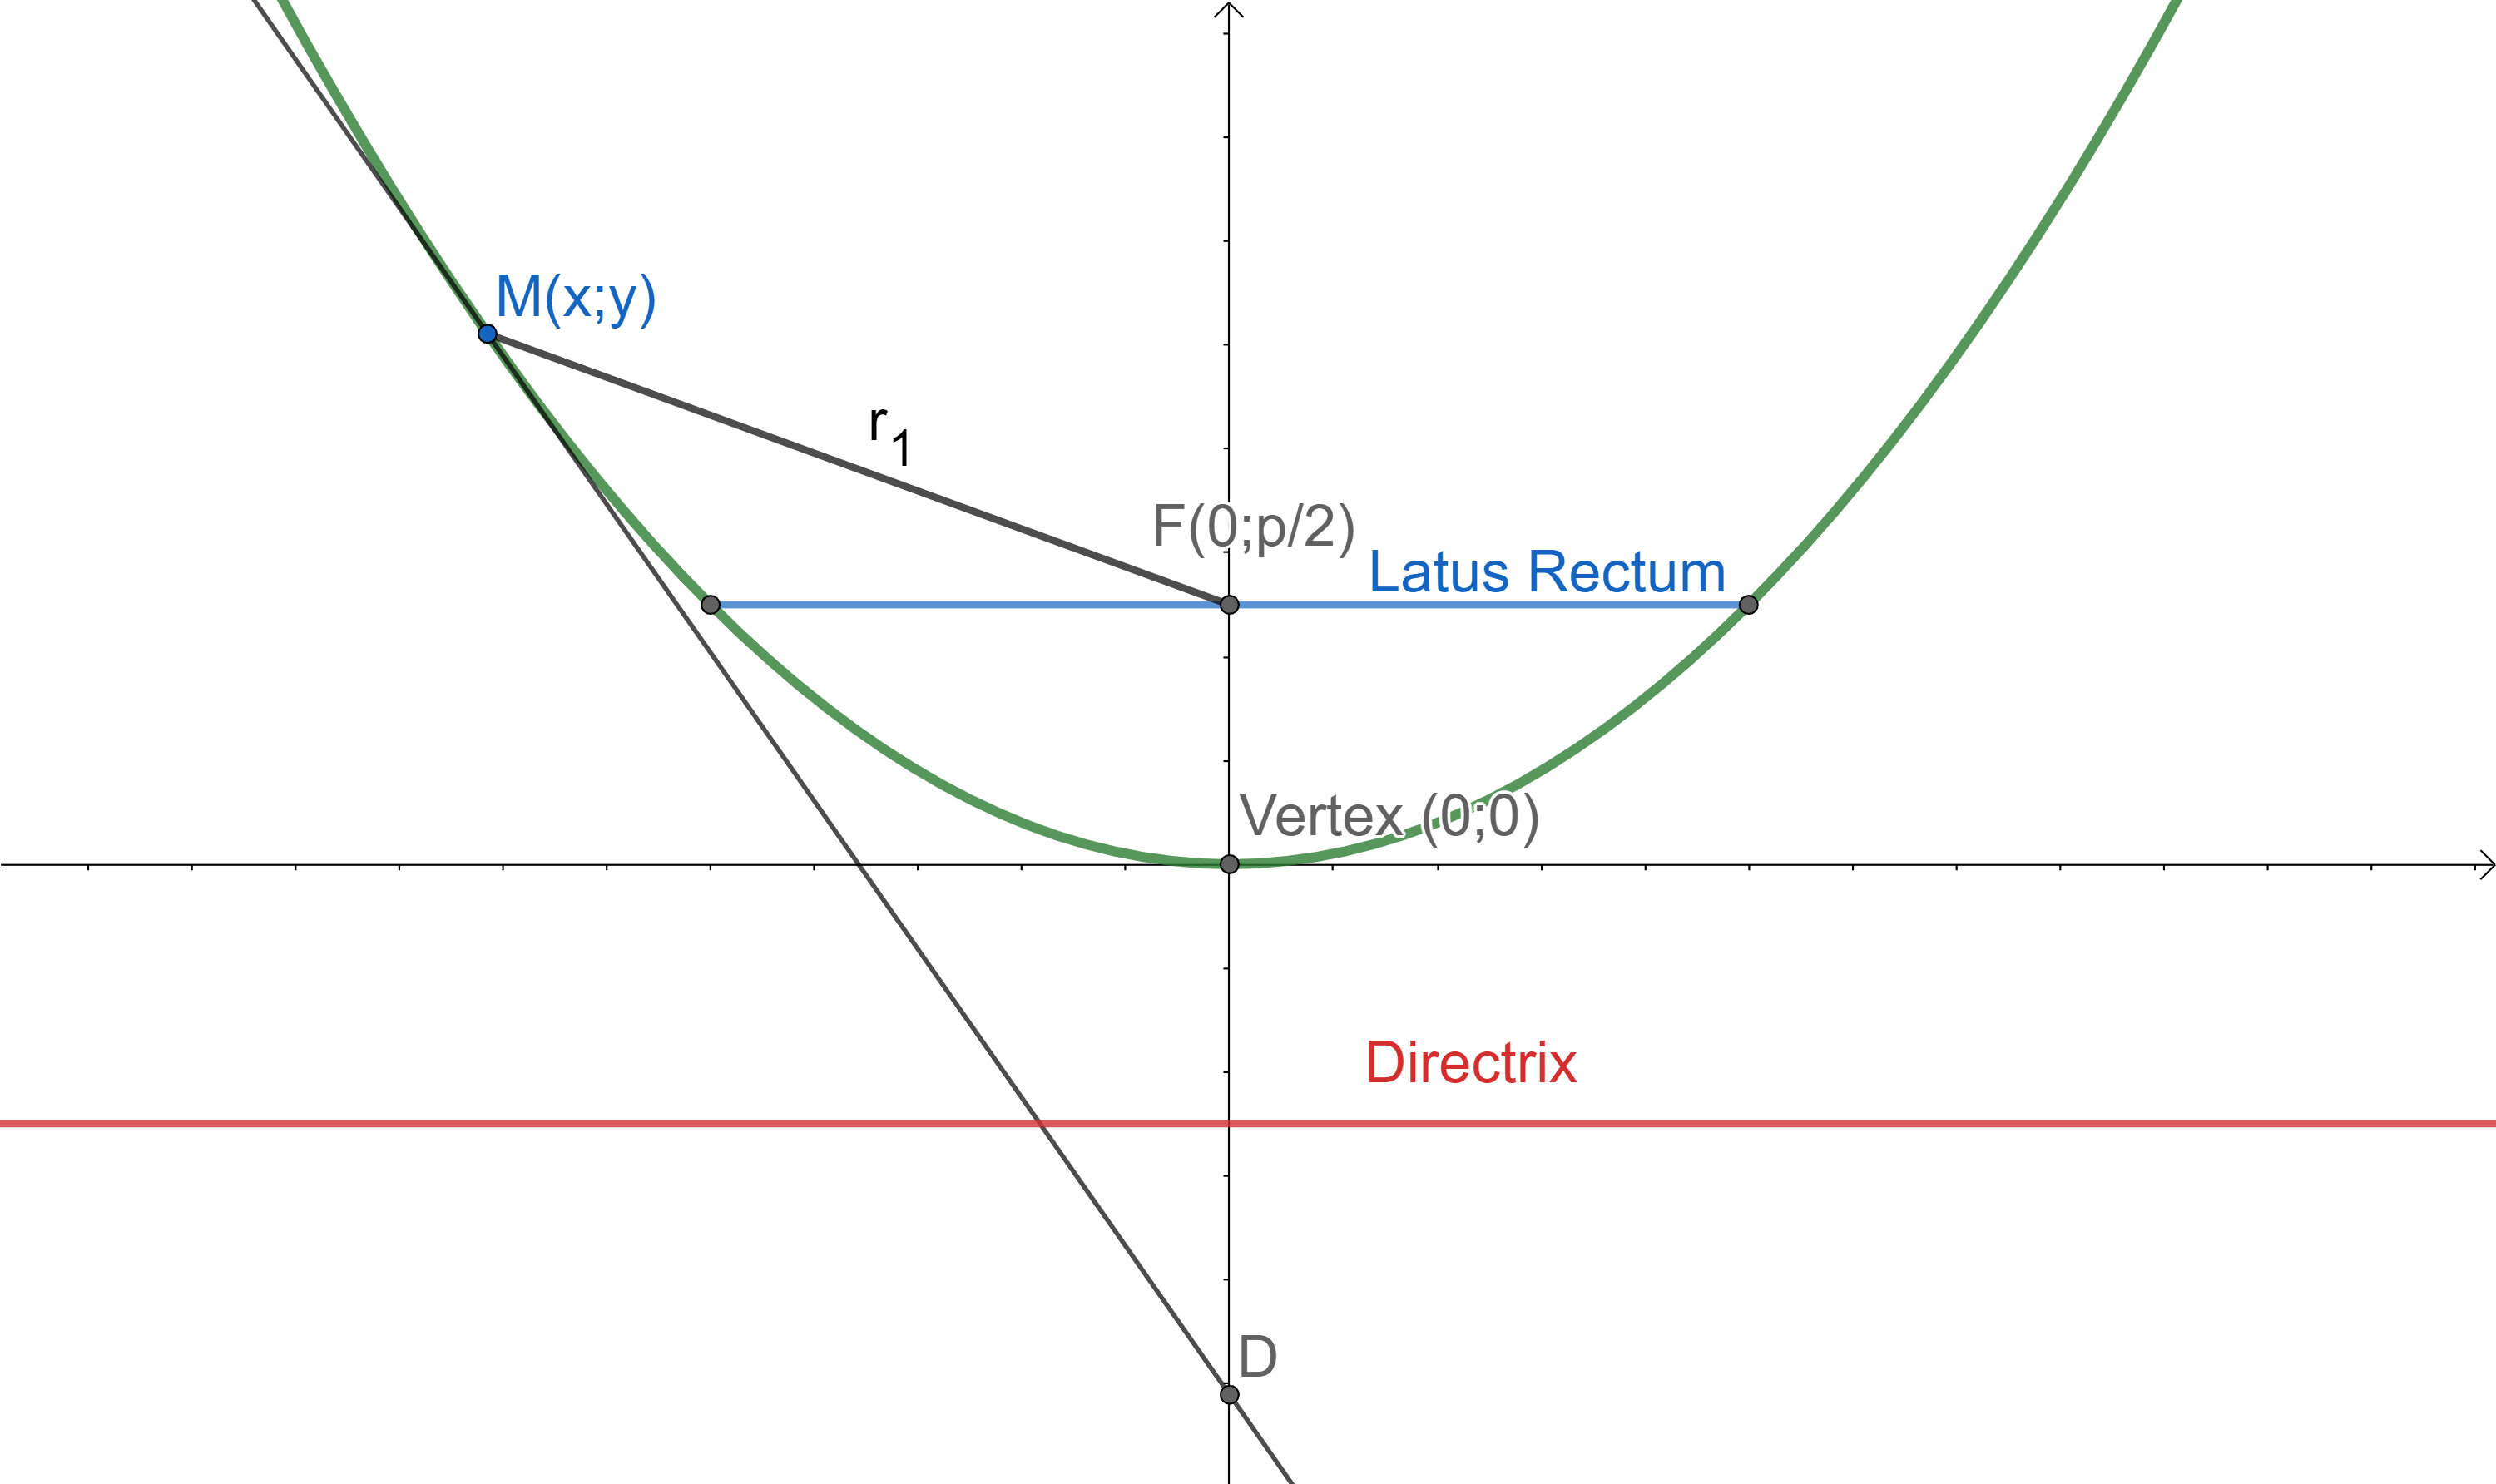
\includegraphics[height=3cm,width=1\textwidth,keepaspectratio]{Parabola.png}
                \vspace{-0.5cm}
                \caption*{\scriptsize Parabola $y=x^2$, $p=\dfrac{1}{2}$}
                \label{fig:Parabola.png}
            \end{figure}
        \end{column}
    \end{columns}
    \vspace{-0.6cm}
    \textit{Properties:}
    \begin{multicols}{3}
        \begin{itemize}
            \item \textbf{Vertex} $\begin{pmatrix} 0\\0 \end{pmatrix} + \begin{pmatrix} x_{\shf}\\y_{\shf} \end{pmatrix}$
            \item \textbf{Center} Not defined
            \item \textbf{Eccentricity} $e = 1$
            \item \textbf{Linear Eccentricity} Not defined
            \item \textbf{Foci} $F = \begin{pmatrix} 0\\\frac{p}{2} \end{pmatrix} + \begin{pmatrix} x_{\shf}\\y_{\shf} \end{pmatrix}$
            \item \textbf{Latus Rectum} (length of chord) $|2p|$
            \item \textbf{Focal parameter}  $p$
            \item \textbf{Discriminant} $\mathfrak{D} = B^2 - 4AC = 0$
            \item \textbf{Directrix eq.} $y = -\frac{p}{2} + y_{\shf}$
            \item \textbf{Tangent eq.}  $x(x_{\text{tan}}-x_{\shf})=p(y-y_{\text{tan}})+x_{\text{tan}}(x_{\text{tan}}-x_{\shf})$
            \item $r = |\overline{FM}|=\sqrt{(x-\frac{p}{2})^2+y^2}$
            \item $\triangle MFD$ is isosceles, where $MD$ -- tangent to $M$
            \end{itemize}
    \end{multicols}
    \end{frame}


    \begin{frame}[t]{Ellipse}
        \framesubtitle{}
            \scriptsize
            \vspace{-0.4cm}
        \begin{columns}[T,onlytextwidth]
            \begin{column}{0.59\textwidth}
                \textit{Forms:} \\
                \begin{itemize}
                    \item \textbf{Canonical (should be w/o shift)} $\frac{(x-x_{\shf})^2}{a^2}+\frac{(y-y_{\shf})^2}{b^2}=1$
                    \item \textbf{General} $Ax^2+Bxy+Cy^2+Dx+Ey+F=0$, where $AC > 0$, if $B=0$
                    \item \textbf{Parametric} $\left\{\begin{matrix*}[l] x = a\cos(\alpha)\\ y = b\sin(\alpha) \end{matrix*}\right.$
                \end{itemize}
            \end{column}
            \begin{column}{0.39\textwidth}
                \vspace{-0.5cm}
                \begin{figure}[H]
                    \centering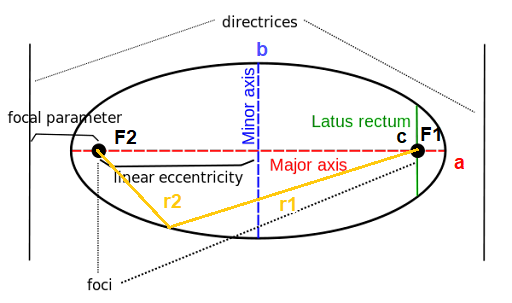
\includegraphics[height=3cm,width=1\textwidth,keepaspectratio]{Ellipse.png}
                    \vspace{-0.5cm}
                    \caption*{\scriptsize Ellipse $\frac{x^2}{a^2}+\frac{y^2}{b^2}=1$}
                    \label{fig:Ellipse.png}
                \end{figure}
            \end{column}
        \end{columns}
        \vspace{-0.5cm}
        \textit{Properties:}
        \vspace{-0.2cm}
        \begin{multicols}{3}
            \begin{itemize}
                \item \textbf{Vert} $\begin{pmatrix} \pm a\\0 \end{pmatrix}$\&$\begin{pmatrix} 0\\\pm b \end{pmatrix}$ $ + \begin{pmatrix} x_{\shf}\\y_{\shf} \end{pmatrix}$
                \item \textbf{Center} $(0;0) + (x_{\shf};y_{\shf})$
                \item \textbf{Eccentricity} $0 \leq e < 1$, $e = \sqrt{1 - \frac{b^2}{a^2}}$
                \item \textbf{Linear Eccentricity} $c = \sqrt{a^2-b^2}$
                \item \textbf{Foci} $F = \begin{pmatrix} \pm(c= e\ a)\\ 0 \end{pmatrix} + \begin{pmatrix} x_{\shf}\\y_{\shf} \end{pmatrix}$
                \item \textbf{Latus Rectum} (length of chord) $\frac{2b^2}{a}$
                \item \textbf{Focal parameter}  $\frac{b^2}{\sqrt{a^2-b^2}}$
                \item \textbf{Discriminant} $\mathfrak{D} = B^2 - 4AC < 0$
                \item \textbf{Directrix eq.} $x = \pm \frac{a}{e} + x_{\shf}$
                \item \textbf{Tangent eq. (w/o shift)} $\dfrac{x_{tangent} x}{a^2}+\dfrac{y_{tangent} y}{b^2}=1$
                \item $r_1 + r_2 = 2a$
                \item $r_{1,2} = |\overline{F_{1,2}M}|=\sqrt{(x \pm c)^2+y^2}$
                \item $\frac{r_1}{d_1}=e$
                \end{itemize}
        \end{multicols}
        \end{frame}

    \begin{frame}[t]{Hyperbola}
        \framesubtitle{}
            \scriptsize
            \vspace{-0.4cm}
        \begin{columns}[T,onlytextwidth]
            \begin{column}{0.59\textwidth}
                \textit{Forms:} \\
                \begin{itemize}
                    \item \textbf{Canonical (should be w/o shift)} $\frac{(x-x_{\shf})^2}{a^2}-\frac{(y-y_{\shf})^2}{b^2}=1$
                    \item \textbf{General} $Ax^2+Bxy+Cy^2+Dx+Ey+F=0$, where $AC < 0$
                    \item \textbf{Parametric} $\left\{\begin{matrix*}[l] x = \dfrac{a}{\cos(\alpha)}\\ y = b\tan(\alpha) \end{matrix*}\right.$
                \end{itemize}
            \end{column}
            \begin{column}{0.39\textwidth}
                \vspace{-0.5cm}
                \begin{figure}[H]
                    \centering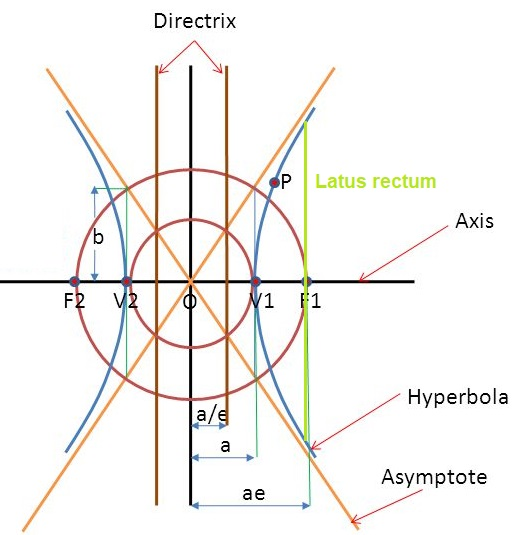
\includegraphics[height=3cm,width=1\textwidth,keepaspectratio]{Hyperbola.jpg}
                    \vspace{-0.4cm}
                    \caption*{\scriptsize Hyperbola $\frac{x^2}{a^2}-\frac{y^2}{b^2}=1$}
                    \label{fig:Hyperbola.jpg}
                \end{figure}
            \end{column}
        \end{columns}
        \vspace{-0.7cm}
        \textit{Properties:}
        \begin{multicols}{3}
            \begin{itemize}
                \item \textbf{Vertex} $\begin{pmatrix} \pm a\\0 \end{pmatrix} + \begin{pmatrix} x_{\shf}\\y_{\shf} \end{pmatrix}$ 
                \item \textbf{Center} $(0;0) + (x_{\shf};y_{\shf})$
                \item \textbf{Eccentricity} $e > 1$, $e = \sqrt{1 + \frac{b^2}{a^2}}$
                \item \textbf{Linear Eccentricity} $c = \sqrt{a^2+b^2}$
                \item \textbf{Foci} $F = \begin{pmatrix} \pm c = \pm (e\ a)\\ 0 \end{pmatrix} + \begin{pmatrix} x_{\shf}\\y_{\shf} \end{pmatrix}$
                \item \textbf{Latus Rectum} $\frac{2b^2}{a}$
                \item \textbf{Focal parameter}  $\frac{b^2}{\sqrt{a^2+b^2}}$
                \item \textbf{Discriminant} $\mathfrak{D} = B^2 - 4AC > 0$
                \item \textbf{Directrix eq.} $x = \pm \frac{a}{e} + x_{\shf}$
                \item \textbf{Asymptots eq.} $y = \pm \frac{b}{a}(x-x_{\shf}) + y_{\shf}$
                \item \textbf{Tangent eq. (w/o shift)} $\dfrac{x_{tangent} x}{a^2}-\dfrac{y_{tangent} y}{b^2}=1$
                \item $r = |\overline{F_{closest}M}|=|x\ e - a|$
                \item $\dfrac{r_1}{d_1}=e$
                \end{itemize}
        \end{multicols}
        \end{frame}

\begin{frame}[t]{Task 1}
    \framesubtitle{}
    \only<1>{
   Find the centre and eccentricity of the hyperbola $9x^2-4y^2+18x+16y-43=0$}
    \only<2>{
        \alert{\Large Answer}
        \begin{figure}[H]
            \centering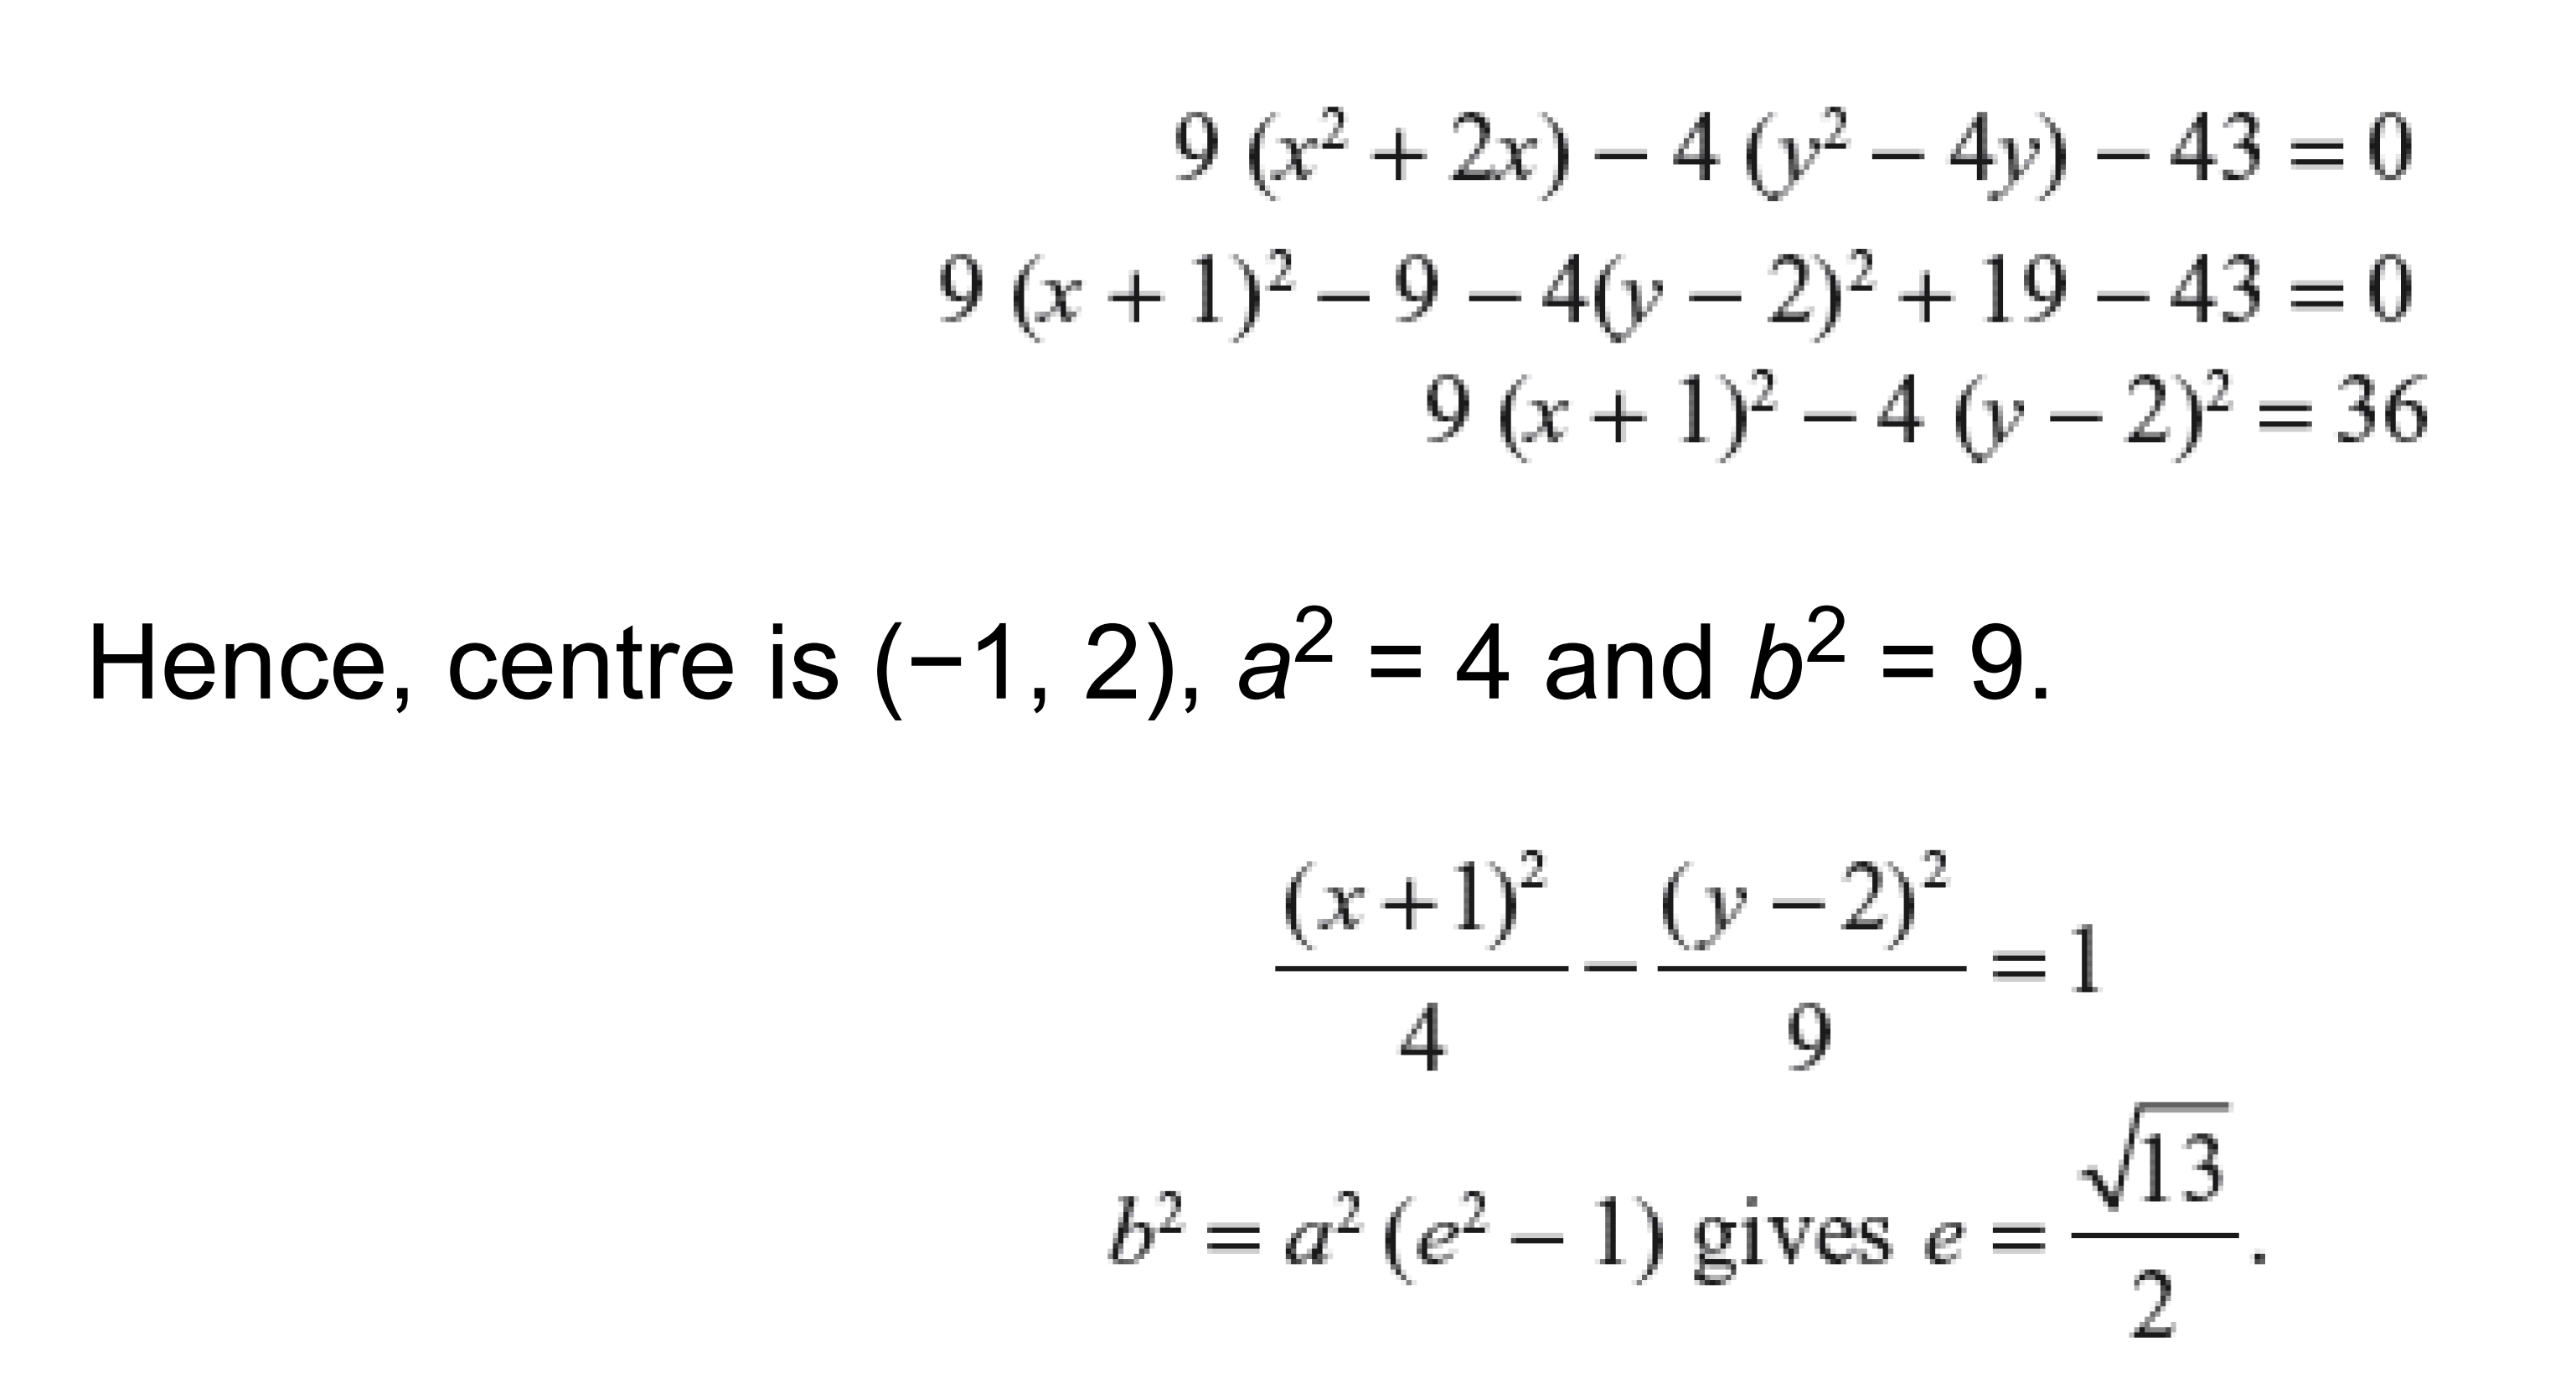
\includegraphics[height=5.5cm,width=1\textwidth,keepaspectratio]{1ans.png}
            % \caption{caption_name}
            \label{fig:1ans.png}
        \end{figure}
    }
\end{frame}

    \begin{frame}[t]{From general to canonical form}
        \framesubtitle{Special case: when $B=0$}
            $Ax^2 +Cy^2 +2Dx + 2Ey +F = 0$ --- General form. \medskip
        
            Example of transformation from general to canonical form:
            \begin{align*}
                16x^2 + 25y^2 - 32x + 50y -359 = 0 \Rightarrow \\
                (16x^2 - 32x) + (25y^2 +50y) -359 = 0 \Rightarrow \\ 
                16(x^2 - 2x) + 25(y^2 + 2y) = 359 \Rightarrow \\ 
                16(x^2 -2x +1) + 25(y^2 +2y +1) = 350 + 16 + 25 \Rightarrow \\
                16(x-1)^2 +25(y+1)^2 = 400 \Rightarrow \\ 
                \frac{(x-1)^2}{25}+\frac{(y+1)^2}{16}=1
            \end{align*}
        \end{frame}

\begin{frame}[t]{From general to canonical form}
\framesubtitle{General case: classical method}
\scriptsize
\vspace{-0.2cm}
        \textbf{Algorithm}
        \begin{enumerate}
            \item Find angle of rotation, using $(A-C)\sin(2\alpha) + B\cos(2\alpha)=0$. If bad angle, try to do the following: \medskip

             $\cot(2\alpha)=\dfrac{A-C}{B}$; $\cos(2\alpha)=\cos(\operatorname{arccot}(2\alpha))=\dfrac{A-C}{\sqrt{(A-C)^2+B^2}}$ $\rightarrow$ $\left\{\begin{matrix*}[l] \cos(\alpha)=\frac{\sqrt{2}}{2}\sqrt{1+\cos(2\alpha)}
            \\ \sin(\alpha)=\frac{\sqrt{2}}{2}\sqrt{1-\cos(2\alpha)}
            \end{matrix*}\right.$
            \item Using roration matrix, write down a transformation from $\begin{bmatrix}x\\y\end{bmatrix} \rightarrow \begin{bmatrix}x'\\y'\end{bmatrix}$; $\begin{bmatrix}x\\y\end{bmatrix} = \begin{bmatrix}
            x'\cos(\alpha) - y'\sin(\alpha)\\ 
            x'\sin(\alpha) + y'\cos(\alpha) 
            \end{bmatrix}$
            \item Substitute it to original equation and simplify to a canonical equation with shifting \\ (for instance, $\dfrac{(x'+x_{shift})^2}{2}+\dfrac{(y'+y_{shift})^2}{8}=1$)
            \item Change the variables again ($\begin{bmatrix}x'\\y'\end{bmatrix} \rightarrow \begin{bmatrix}x''\\y''\end{bmatrix}$; $\begin{bmatrix}x''\\y''\end{bmatrix} = \begin{bmatrix}x' + x_{shift}\\y'+y_{shift}\end{bmatrix}$). It gives you a canonical form.
            \item Write a system which shows $\begin{bmatrix}x''\\y''\end{bmatrix} = \begin{bmatrix}f(x,y)\\g(x,y)\end{bmatrix}$. You need to agregate (2) and (4) to (5)
        \end{enumerate}
\end{frame}

\begin{frame}[t]{From general to canonical form}
\framesubtitle{Classical method: case study (1)}
    \vspace{-0.6cm}
    \begin{figure}[H]
        \centering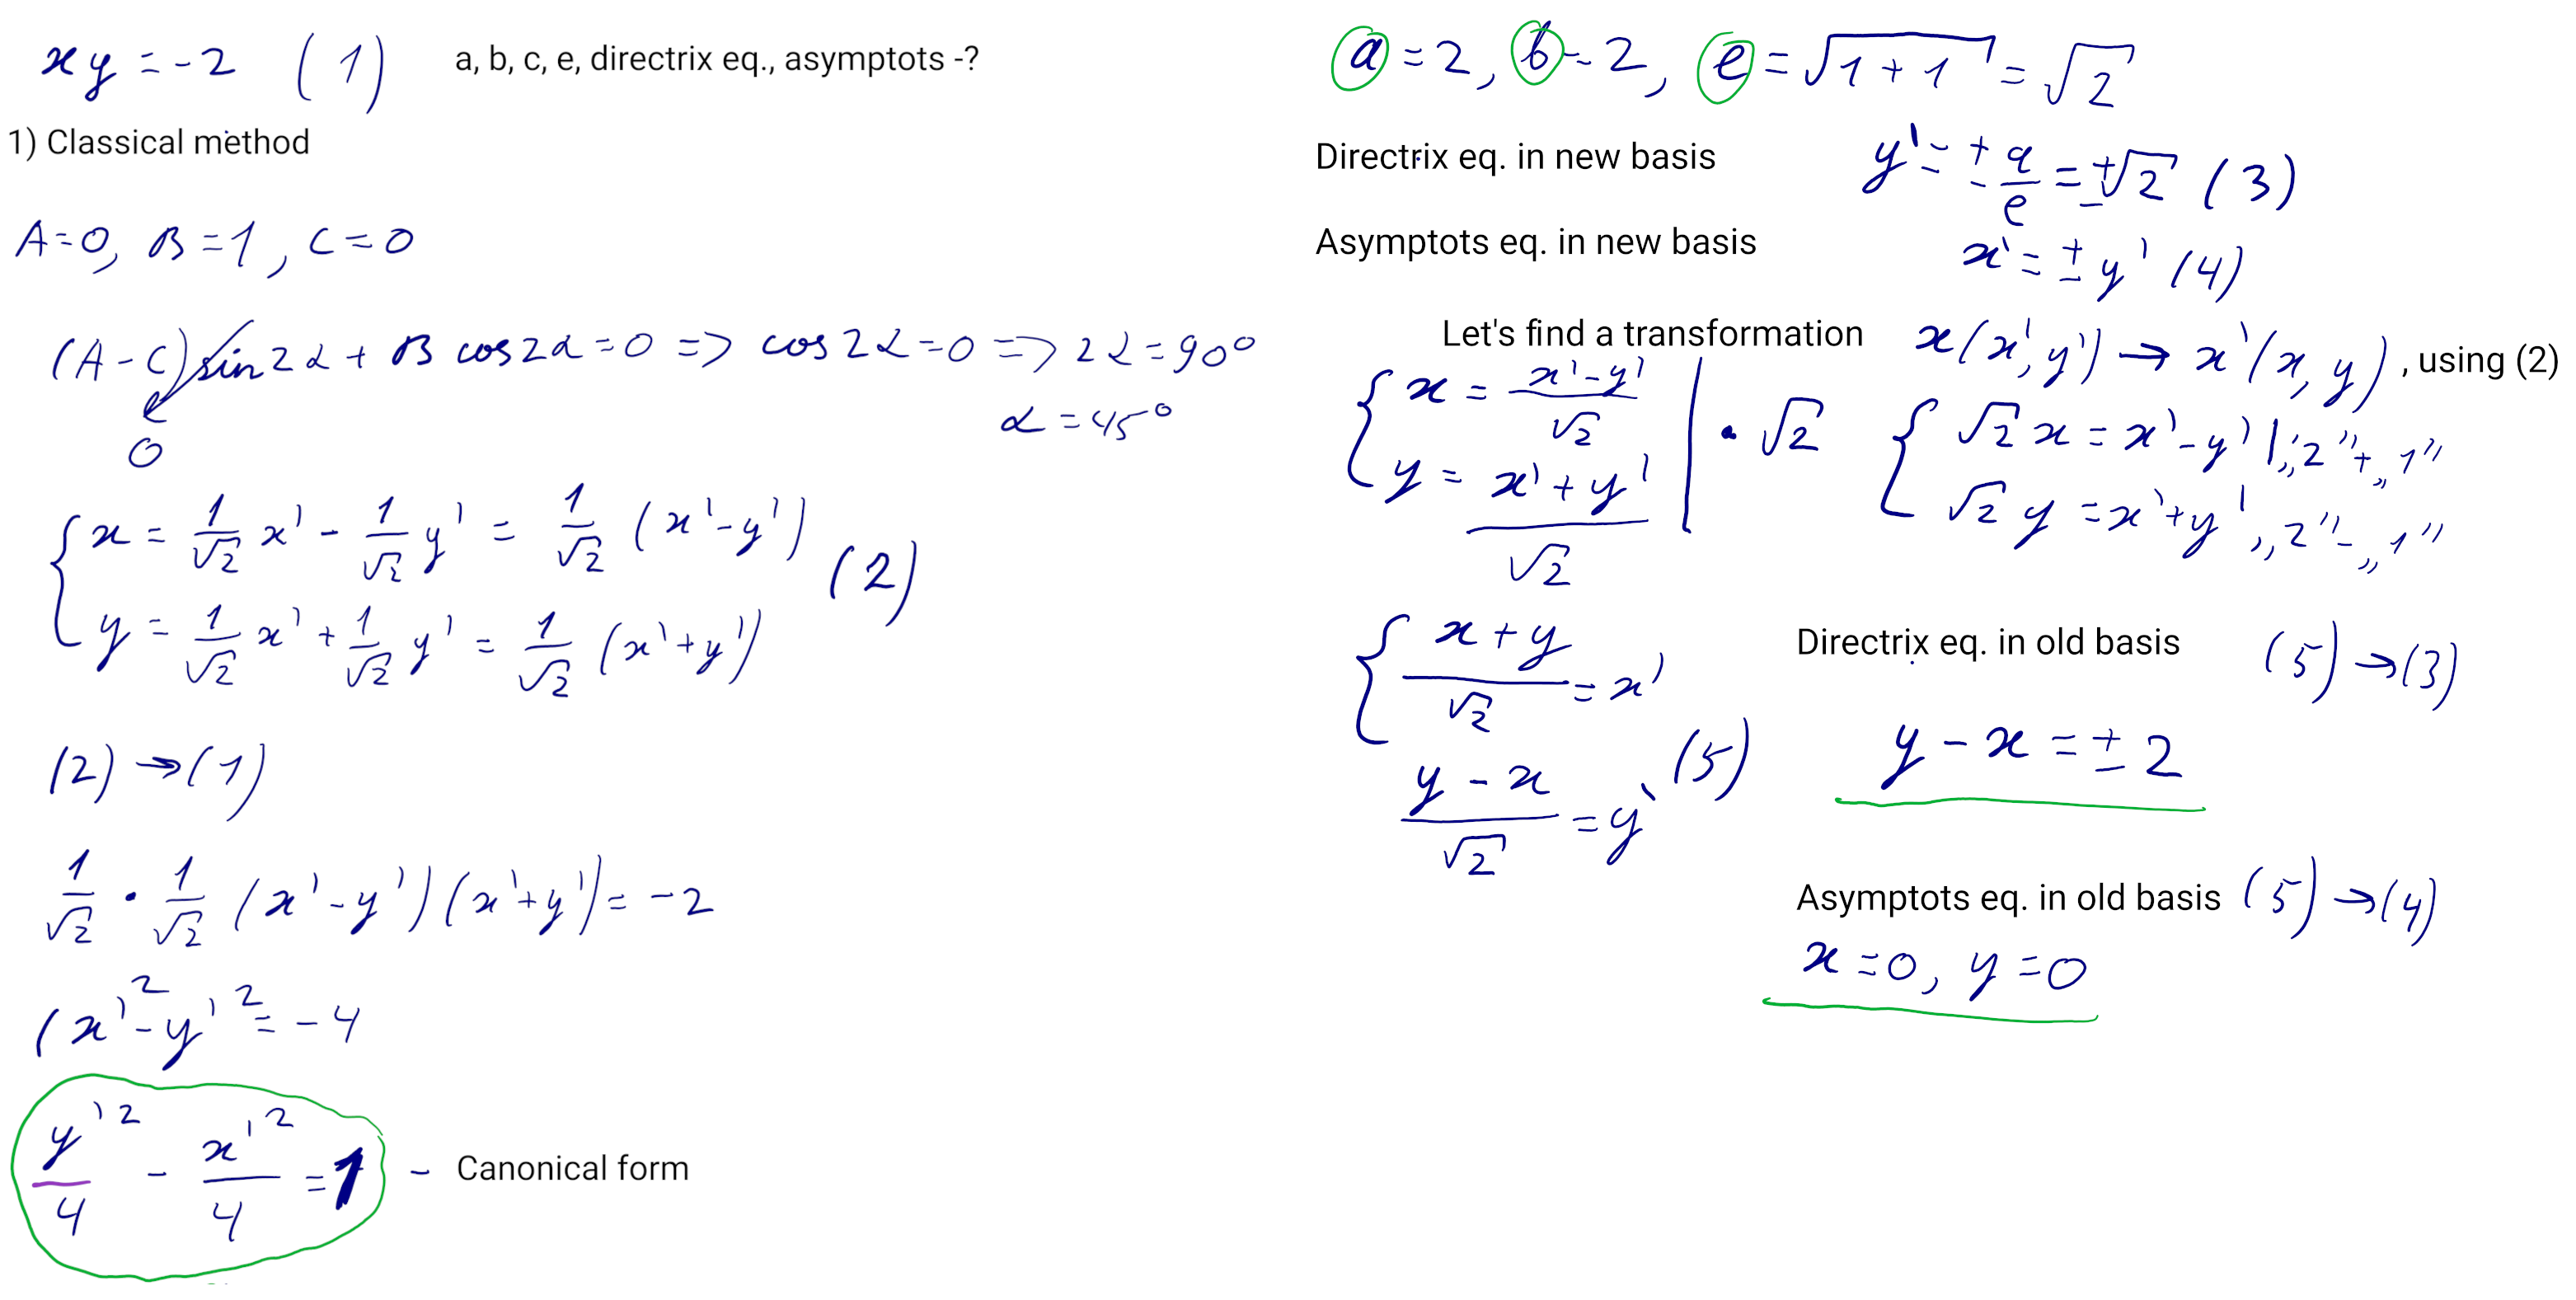
\includegraphics[height=6cm,width=1\textwidth,keepaspectratio]{classic.png}
        \label{fig:classic.png}
    \end{figure}
\end{frame}

\begin{frame}[t]{From general to canonical form}
\framesubtitle{General case: Other way}
\scriptsize
\vspace{-0.3cm}
\textbf{Problem}\\
In some cases it's quite tough to convert from general form to canonical using classical method from the class (bad numbers).\\
\textbf{Solution} \smallskip
\begin{columns}[onlytextwidth]
\column{0.47\textwidth}
$f = Ax^{2}+Bxy+Cy^{2}+Dx+Ey+F=0$ \\
converts into canonical form in new variables ${x''}$, ${y''}$ by the equation:
$
    {\dfrac {{({x}'')}^{2}}{-S/(\lambda _{1}^{2}\lambda _{2})}}+{\dfrac {{({y}'')}^{2}}{-S/(\lambda _{1}\lambda _{2}^{2})}}=1
$, where \\
\begin{itemize}
    \item $S$ is determinant of $\left({\begin{matrix}A&B/2&D/2\\B/2&C&E/2\\D/2&E/2&F\end{matrix}}\right)$ matrix 
\item $\lambda_{1,2}$ are the eigenvalues of  $\left({\begin{matrix}A&B/2\\B/2&C\end{matrix}}\right)$ matrix.\\
It can be found using this equation:
$
    \lambda ^{2}-(A+C)\lambda +(AC-(B/2)^{2})=0
$
\end{itemize}
\column{0.52\textwidth}
Using \textit{canonical form}, we can find $a,\ b,\ c,\ e$ for the curve, but not \textit{coordinate dependent properties (like vertex, directrix eq.)}.

For this purpose, we need to find \textbf{angle} and \textbf{shift}.\\
\textbf{Angle}: $(A-C)\sin(2\alpha) + B\cos(2\alpha) = 0; \rightarrow \alpha = ...$

\textbf{Shift (center of the curve)}
\begin{equation*}
    \left\{\begin{matrix*}[l] \frac{\partial f}{\partial x}\\ \frac{\partial f}{\partial y} \end{matrix*}\right. \rightarrow \text{2 equations of line} \rightarrow \text{solve system } (x_c;y_c)
\end{equation*}

Using this transformation, we can find original coordinates, knowing the new one
\begin{equation*} \begin{bmatrix}
x_A\\ y_A \\1
\end{bmatrix} = 
\begin{bmatrix}
\cos(\alpha) & -\sin(\alpha) & x_c \\ \sin(\alpha) & \cos(\alpha) & y_c \\ 0 & 0 & 1
\end{bmatrix} \begin{bmatrix}
{x}_A''\\{y}_A''\\1
\end{bmatrix}
\end{equation*}
\end{columns}
\end{frame}

\begin{frame}[t]{From general to canonical form}
    \framesubtitle{General case: Other way (2)}
    \vspace{-0.6cm}
    \begin{figure}[H]
        \begin{tikzpicture}[set/.style={fill=cyan,fill opacity=0.1},scale=1.3]
 
            % Help grid
            \draw[black!5,step=0.5] (-1,-3) grid (3,1.5);
             
            % Ellipse 3
            \draw[set,
                xshift=1.5cm,
                yshift=-1.705cm,
                rotate =45] (0,0) ellipse (1cm and 0.5cm);

            \draw[-stealth, very thick,blue] (0,0) -- (1,0)
            node[right,black]{\small $x$};

            \draw[-stealth, very thick,red] (0,0) -- (0,1)
            node[above,black]{\small $y$};

            \draw[xshift=1.5cm, yshift=-1.705cm, rotate =45, -stealth, very thick,blue] (0,0) -- (1,0)
            node[right,black]{\small ${x''}$};

            \draw[xshift=1.5cm, yshift=-1.705cm, rotate =45, -stealth, very thick,red] (0,0) -- (0,1)
            node[above,black]{\small ${y''}$};

            \filldraw[black] (0.75,-2) circle (2pt) node[left]{\small $A$};

            \draw[-stealth, very thick,green] (1.5,-1.705) -- (0.75,-2)
            node[midway,below right=-2pt, black]{\tiny $\begin{bmatrix}{x}_{A}''\\{y}_{A}''\end{bmatrix}$};

            \draw[-stealth, very thick,green] (0,0) -- (0.75,-2)
            node[midway,below left=-2pt, black]{\tiny $\begin{bmatrix}x_{A}\\y_{A}\end{bmatrix}$};
            \end{tikzpicture}
    \end{figure}
\end{frame}

\begin{frame}[t]{From general to canonical form}
\framesubtitle{Other method: case study}
    \vspace{-0.6cm}
    \begin{figure}[H]
        \centering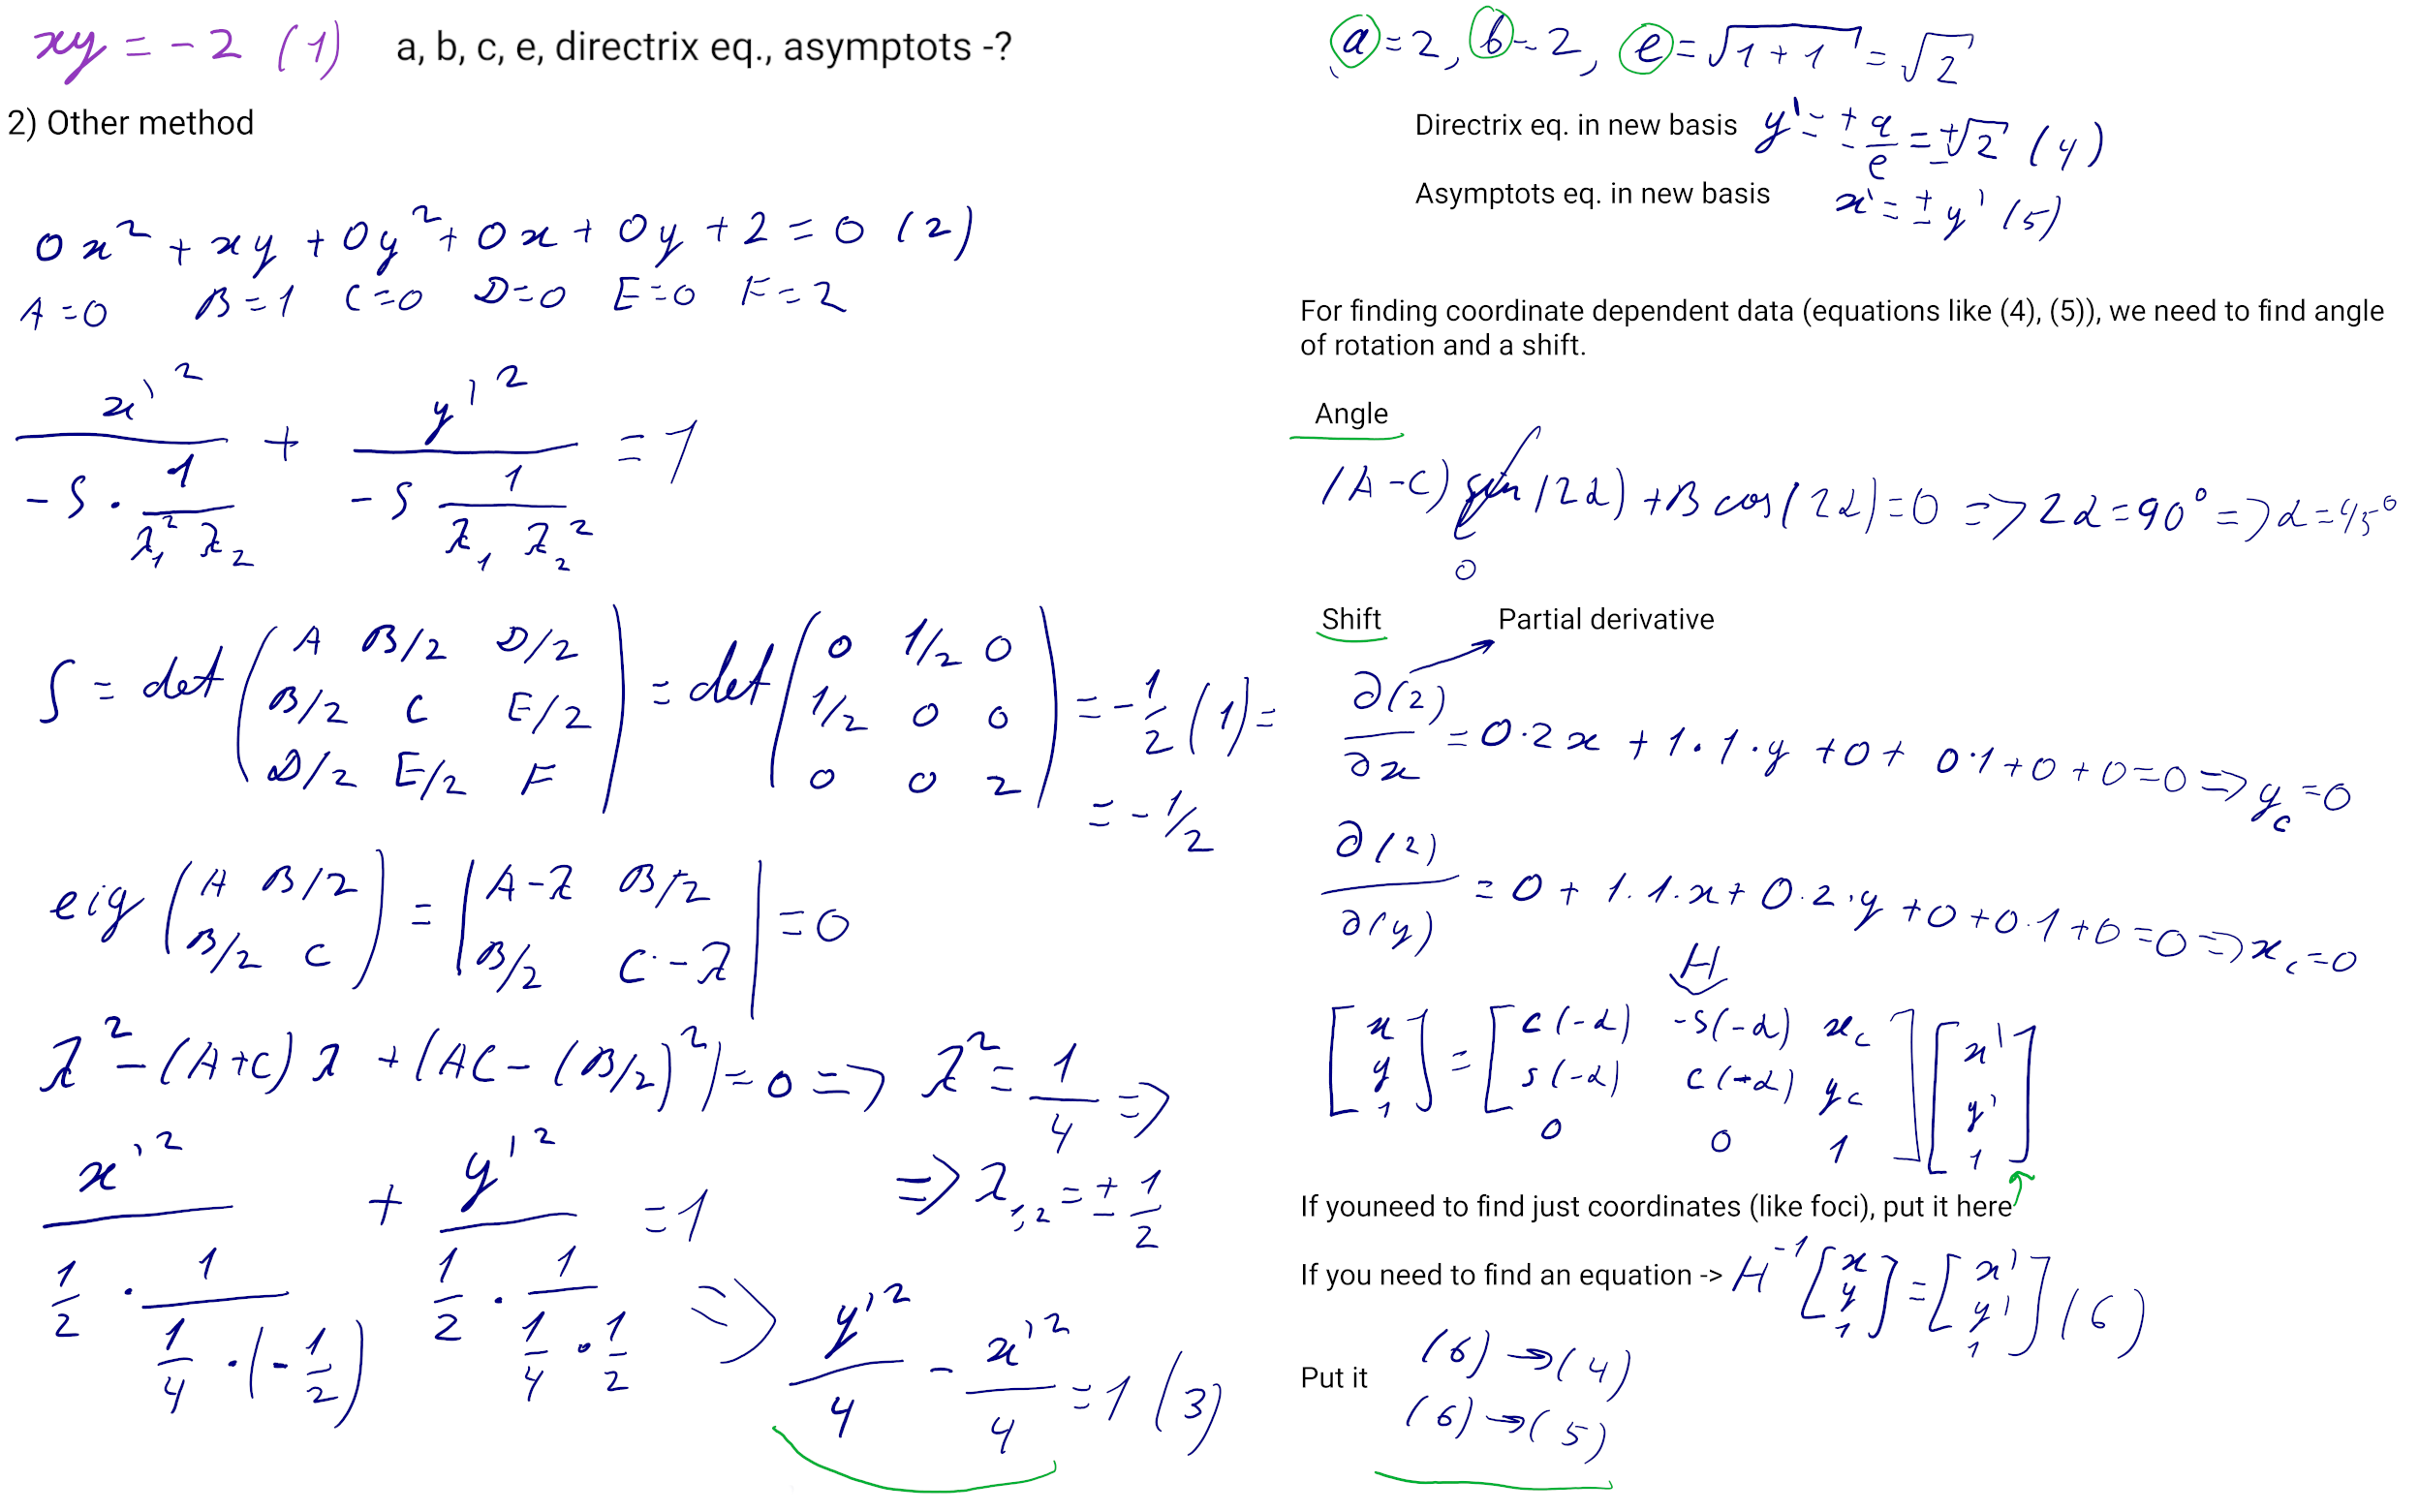
\includegraphics[height=6cm,width=1\textwidth,keepaspectratio]{other.png}
        \label{fig:other.png}
    \end{figure}
\end{frame}

\begin{frame}[t]{Task 2}
    \framesubtitle{}
    \only<1>{Transform $x^2-xy+y^2+x+y=0$ into canonical form}
    \only<2>{
        \alert{\Large Answer}
        \begin{figure}[H]
            \centering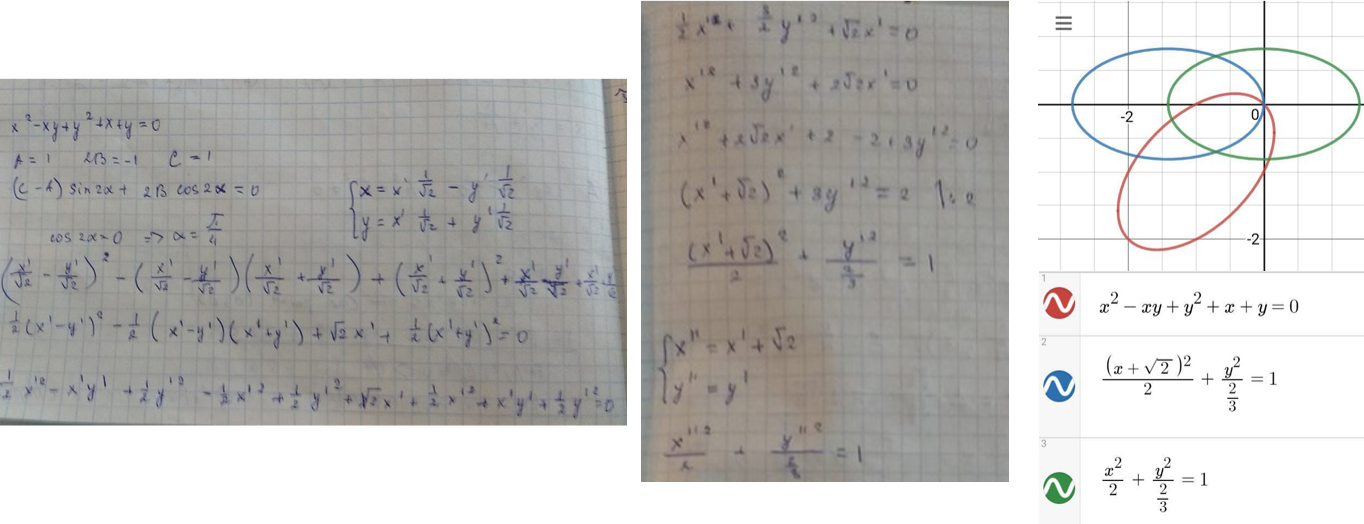
\includegraphics[height=5.5cm,width=1\textwidth,keepaspectratio]{2ans.png}
            % \caption{caption_name}
            \label{fig:2ans.png}
        \end{figure}
    }
\end{frame}

\begin{frame}[t]{Task 3}
    \framesubtitle{}
    \only<1>{Prove that a curve given by $7x^2+48xy-7y^2-62x-34y+98=0$ is a hyperbola. Find the eccentricity of this hyperbola, coordinates of its center and foci. Find the equations of axes, asymptotes and directrices of this hyperbola.}
    \only<2>{
        \alert{\Large Answer}

        Eccentricity is $\sqrt{2}$;\\ center --- $(1;1)$;\\ foci --- $F_1(-\frac{1}{5};\frac{13}{5}),\ F_2(\frac{11}{5};\frac{-3}{5})$;\\ real axis is $4x+3y-7=0$;\\ imaginary axis --- $3x-4y+1=0$; \\directrices are $3x-4y-4=0$ and $3x-4y+6=0$;\\ asymptotes --- $x+7y=9$, $7x-y=6$. 
    }
\end{frame}

\note{Эта задача не имеет красивых чисел и поэтому 2ой способ предпочтительнее.}

\begin{frame}[t]{Task 4}
    \framesubtitle{}
    \only<1>{
Find the equation to the hyperbola that passes through $(2;3)$ and has for its asymptotes the lines $4x+3y-7=0$ and $x-2y=1$
    }
    \only<2>{
        \alert{\Large Answer}
        \begin{figure}[H]
            \centering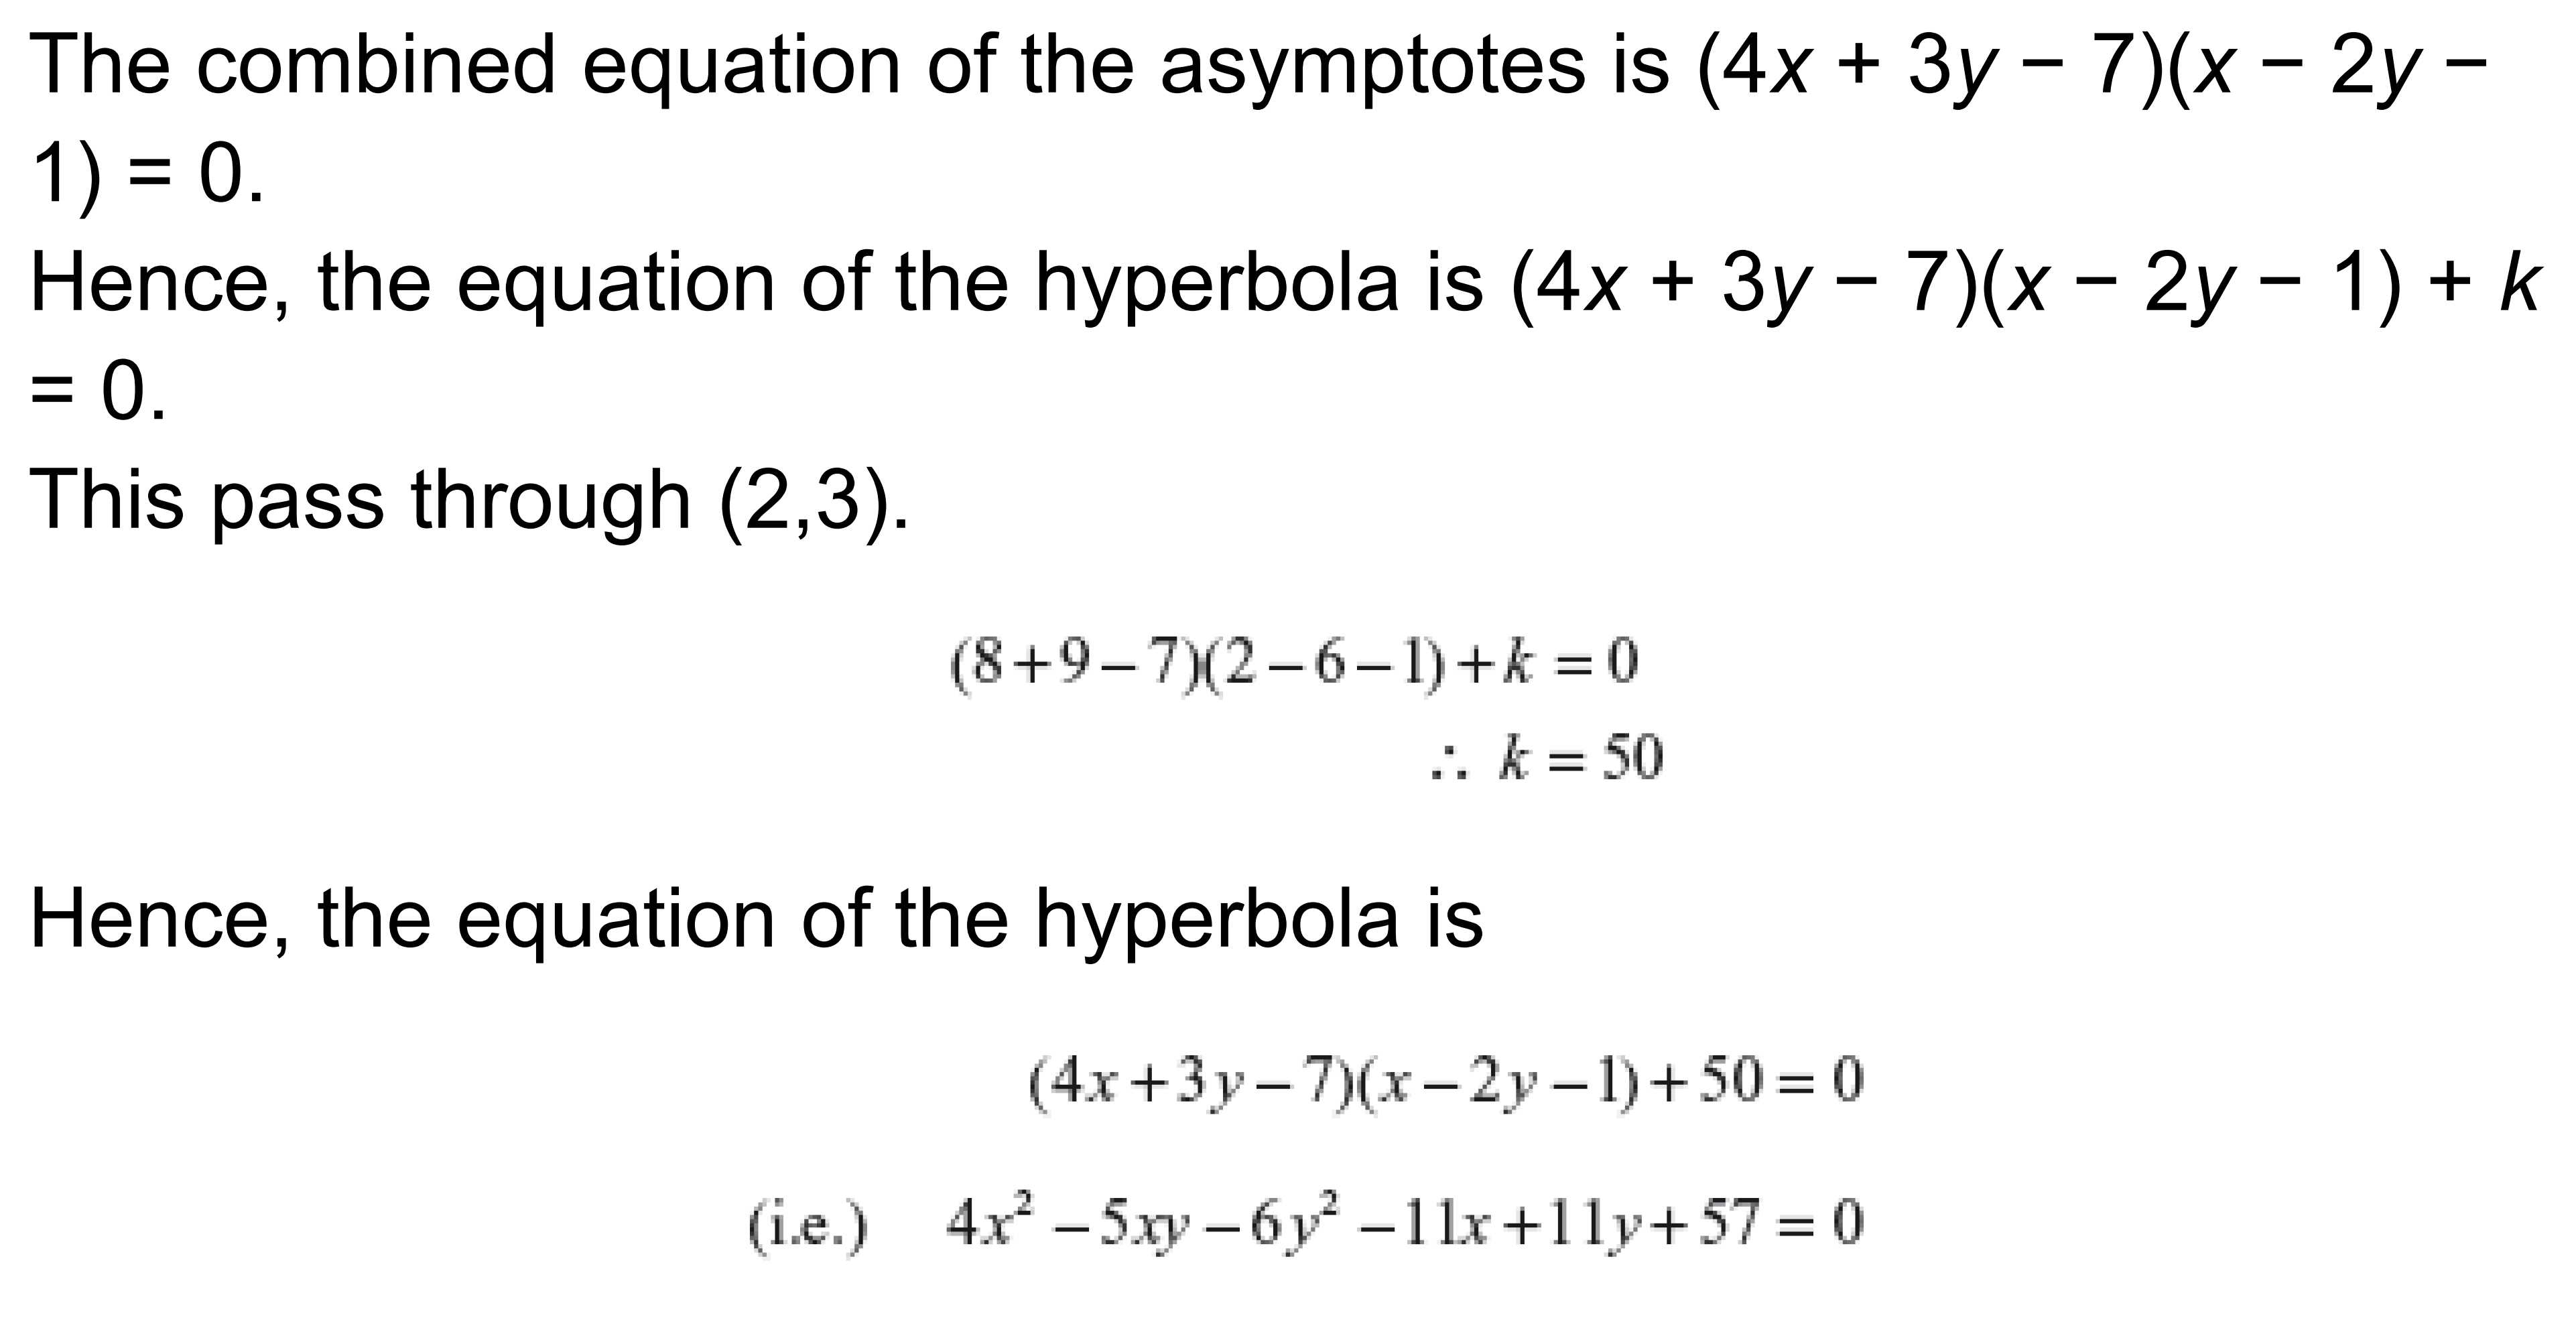
\includegraphics[height=5.5cm,width=1\textwidth,keepaspectratio]{4ans.png}
            % \caption{caption_name}
            \label{fig:4ans.png}
        \end{figure}
    }
\end{frame}

\note{Предложить зареверсить задачу, так как там есть combined equation of asymptotes. Намекнуть, что это можно загуглить и все такое.

По факту тут появляется pair of straight lines. И можно объяснить еще раз, откуда оно тут (сечение в конусе и что из стрейт лайнс появляется гипербола, когда сдвиг проходит).}

\begin{frame}[t]{Task 5}
    \framesubtitle{}
    \only<1>{
        Find the equations of lines tangent to curve $6xy+8y^2-12x-26y+11=0$ that are 

(a) parallel to line $6x+17y-4=0$;

(b) perpendicular to line $41x-24y+3=0$;

(c) parallel to line $y=2$.
    }
    \only<2>{
        \alert{\Large Answer (a)}
        \begin{figure}[H]
            \centering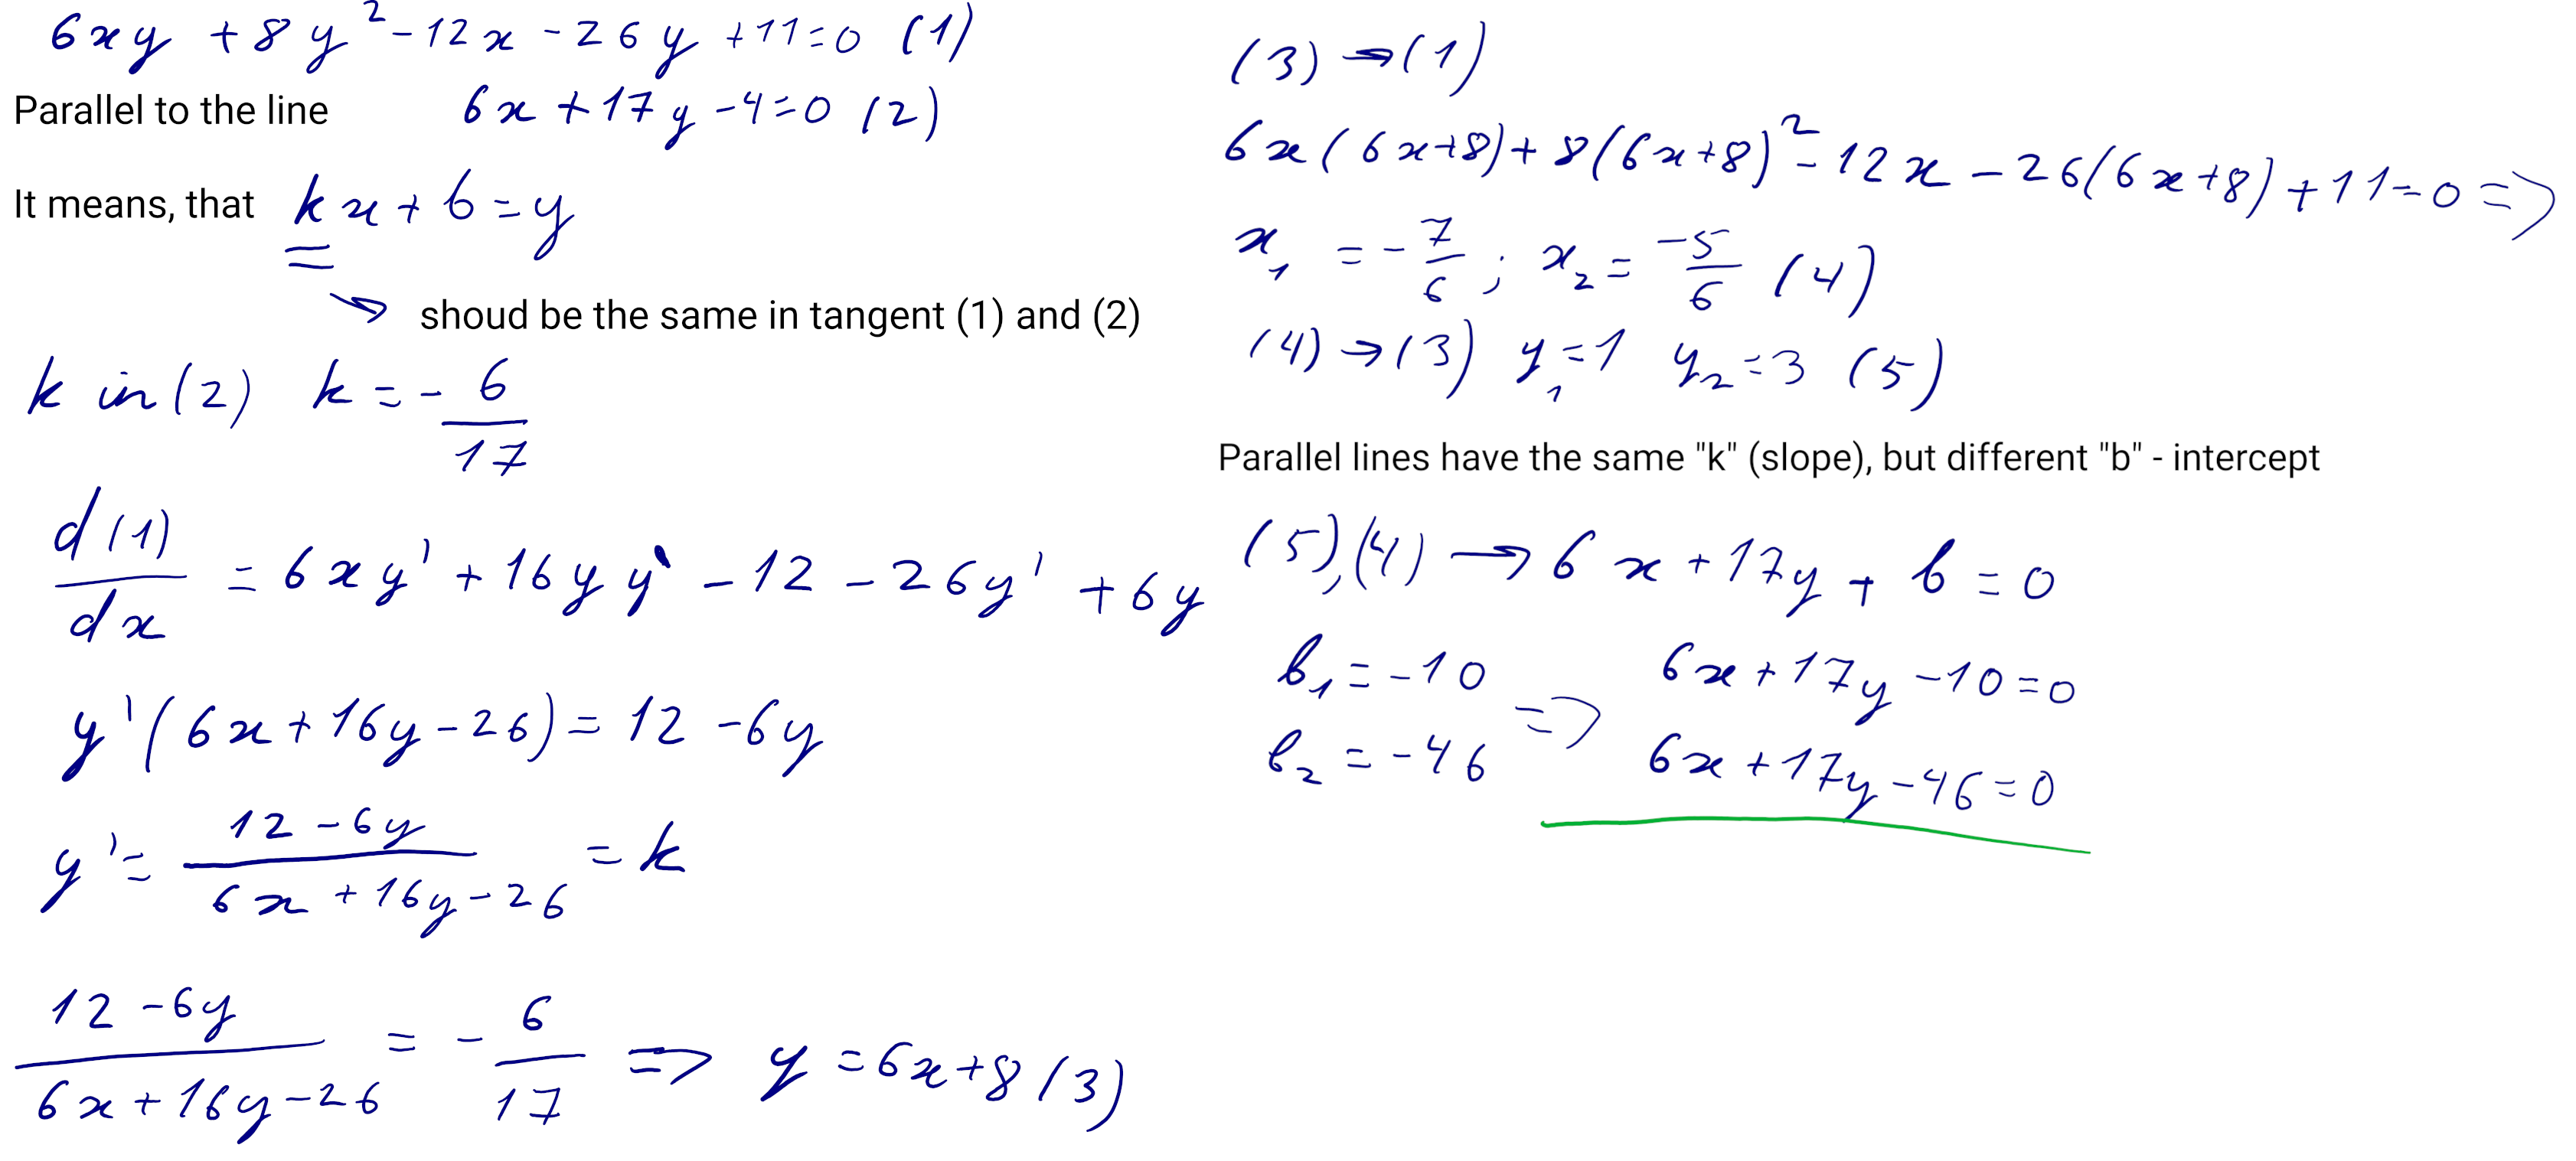
\includegraphics[height=5.5cm,width=1\textwidth,keepaspectratio]{5ans.png}
            % \caption{caption_name}
            \label{fig:5ans.png}
        \end{figure}
    }
    \only<3>{
        \alert{\Large Answer}
        
        (a) $6x + 17y -10 =0$ and $6x +17y -46=0$ \\ 
        (b) $24x + 41y -22=0$ and $24x+41y-94=0$ \\
        (c) no solution
    }
\end{frame}

\begin{frame}[t]{Task 6}
    \framesubtitle{}
    \only<1>{
    Determine types of curves given by the following equations. For each of the curves, find its canonical coordinate system (i.e. indicate the coordinates of origin and new basis vectors in the initial coordinate system) and its canonical equation.
    
(a) $9x^2-16y^2-6x+8y-144=0$;

(b) $9x^2+4y^2+6x-4y-2=0$;

(c) $12x^2-12x-32y-29=0$;

(d) $xy+2x+y=0$;

(e) $5x^2+12xy+10y^2-6x+4y-1=0$;

(f) $8x^2+34xy+8y^2+18x-18y-17=0$;

(g) $25x^2-30xy+9y^2+68x+19=0$;

(h) $x^2+2xy+y^2-5x-5y+4=0$.
    }
    \only<2>{
        \alert{\Large Answer (may contain typos, recommend to check by geogebra)}
        \begin{figure}[H]
            \centering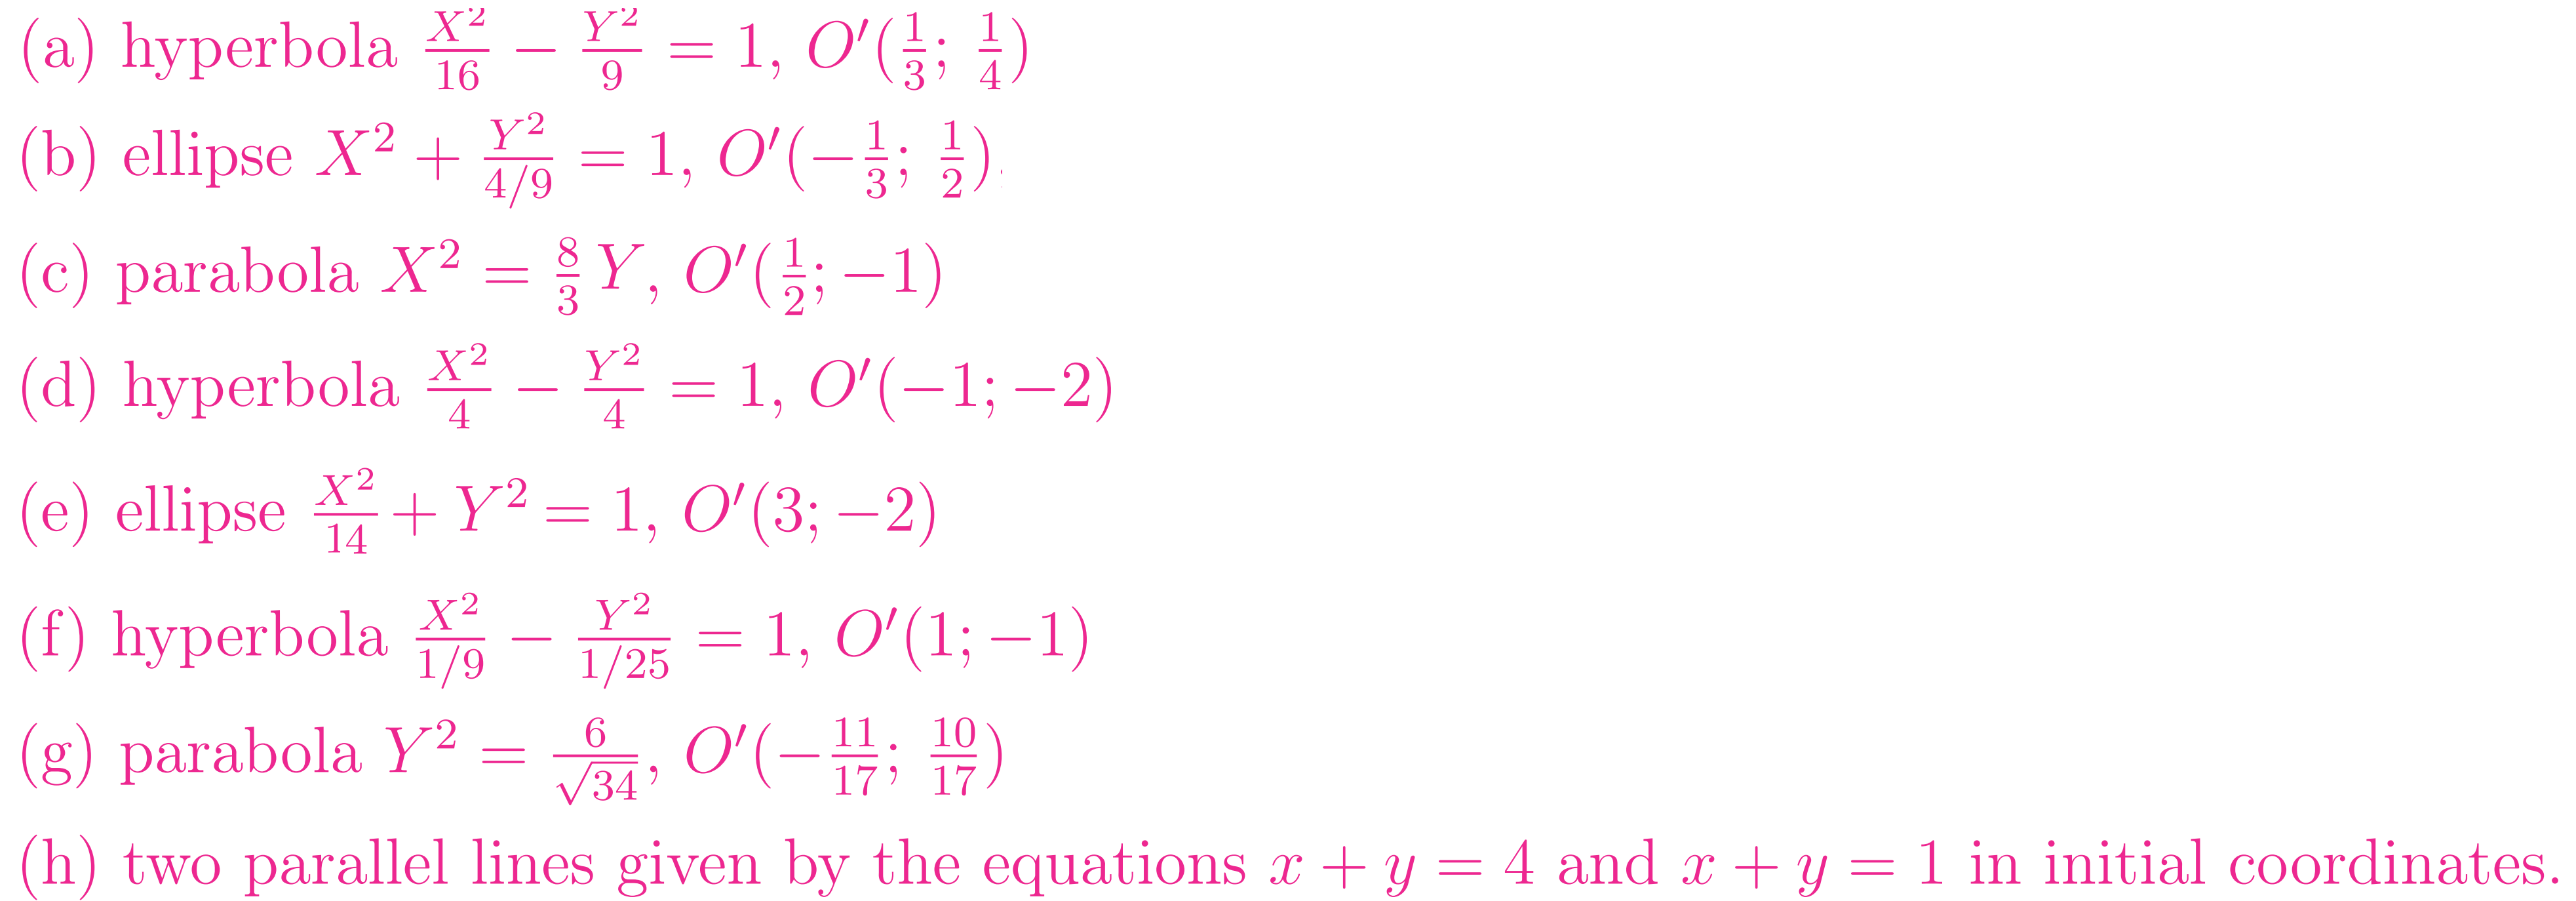
\includegraphics[height=5.5cm,width=1\textwidth,keepaspectratio]{6ans.png}
            % \caption{caption_name}
            \label{fig:6ans.png}
        \end{figure}
    }
\end{frame}

\begin{frame}[t]{Reference material}
    % \framesubtitle{OnlineMschool}
    \Large
    \begin{itemize}
        \item \href{https://ppt-online.org/842240}{Conic sections (slides, rus)}
        \item \href{https://www.youtube.com/watch?v=GaSrBIUGdWs}{How to find centre of conic (video, eng)}
        \item \href{https://math.stackexchange.com/questions/2235355/find-major-and-minor-axis-of-given-conic}{Find the equation of major and minor axis of the given conic}
        \item \href{http://mathprofi.ru/kak_privesti_uravnenie_linii_2_poryadka_k_kanonicheskomu_vidu.html}{How to go from general to canonical form (mathprofi, rus)}
    \end{itemize}
\end{frame}

\fbckg{fibeamer/figs/last_page.png}
\frame[plain]{}

\end{document}